\documentclass{article}
\usepackage{graphicx,fancyhdr,amsmath,amssymb,amsthm,subfig,url,hyperref,epigraph,lipsum}
\usepackage[margin=1in]{geometry}
\setlength\epigraphwidth{.8\textwidth}

% Bibliography
\usepackage[backend=biber, style=authortitle-comp, maxcitenames=1, refsection=section]{biblatex}
\addbibresource{report.bib}

%----------------------- Macros and Definitions --------------------------

\renewcommand{\theenumi}{\bf \Alph{enumi}}

\fancypagestyle{plain}{}
\pagestyle{fancy}
\fancyhf{}
\fancyhead[RO]{\sffamily\large University of Delhi}
\fancyhead[LO]{\sffamily\large MCS-204 Advanced Computer Networks}
\fancyfoot[RO]{\sffamily\thepage}
\renewcommand{\headrulewidth}{1pt}
\renewcommand{\footrulewidth}{1pt}

\graphicspath{{figures/}}

%-------------------------------- Title ----------------------------------

\title{Emerging Trends in Mobile Communications}
\author{
    Samyak Ahuja \\
    \texttt{Class ID: 29}
    \and
    Mayank Kharbanda \\
    \texttt{Class ID: 16}
}

%--------------------------------- Text ----------------------------------

\begin{document}
\maketitle

%--------------------------------- Title ----------------------------------
\section{Li-Fi}

\epigraph{There is a crack in everything.
That's how the light gets in.}{\parencite{selected-poem}}


%---------------------------- Introduction -------------------------------

\subsection{Introduction}

Today, when the world is exploring 5G technology, and smart devices are
connecting to the cloud for fluid communication and IOT.  Daily data traffic is
increasing at the steepest rate. According to \textcite{cisco19} it has been
estimated that, mobile data traffic will reach to 77 exabytes per month by
2022. It is not hidden from the industry that current transmission system is
under pressure.\\

\begin{figure}[!h]
  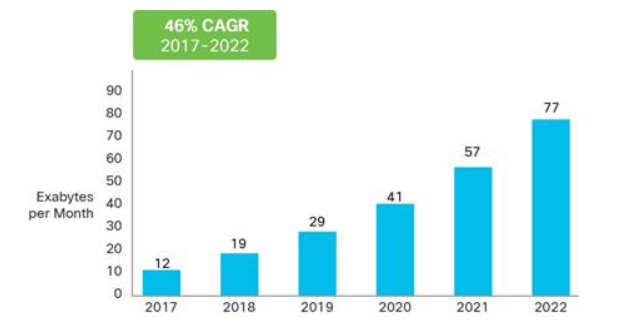
\includegraphics{res/traffic_trend_li_fi.PNG}
    \caption{Mobile data traffic. Source: \parencite{cisco19}}
  \label{fig:traffic_trend_li_fi}
\end{figure}


To revive the radio-wave spectrum from high traffic concentration, a new
technology is attracting scientists, it's Visible light communication using the
concept of Orthogonal Frequency Division Multiplexing(OFDM) or simply termed as
Li-Fi(Light Fidelity).\newline Li-Fi was first introduced to the world by Prof.
Herald Haas during a TEDGLobal Talk in July 2011. In that talk,
\textcite{hass11}, showcased the potential of the technology to be integrated
in the future communication system. From then, scientists from parts of
world started studying for various ways to improve the transmission method.\\

\begin{figure}[!h]
  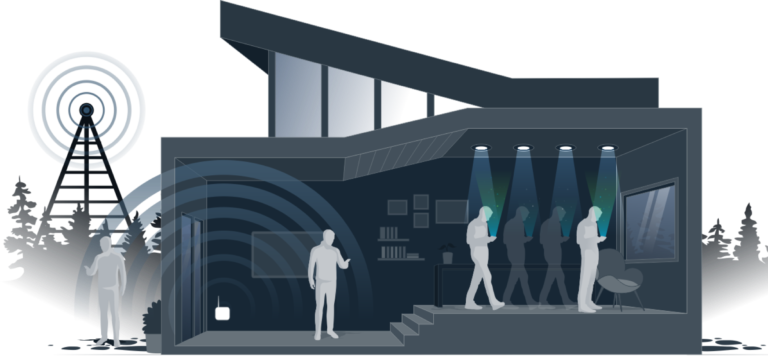
\includegraphics[width=\linewidth]{res/tech-illustration-li-fi.png}
    \caption{Li-Fi. Source: \parencite{purelifi}}
  \label{fig:tech-illustration-li-fi}
\end{figure}


The technology uses visible-light spectrum as a medium for data transmission.
It comprises of a huge bandwidth of 400THz as compared to radio-waves in GHz.
Moreover, visible light does not have any adverse effect on our body as that of
radio-waves. LEDs are perfect candidates for light transmission as they have
the property that their intensity can be changed at a very high speed.


\begin{figure}[!h]
  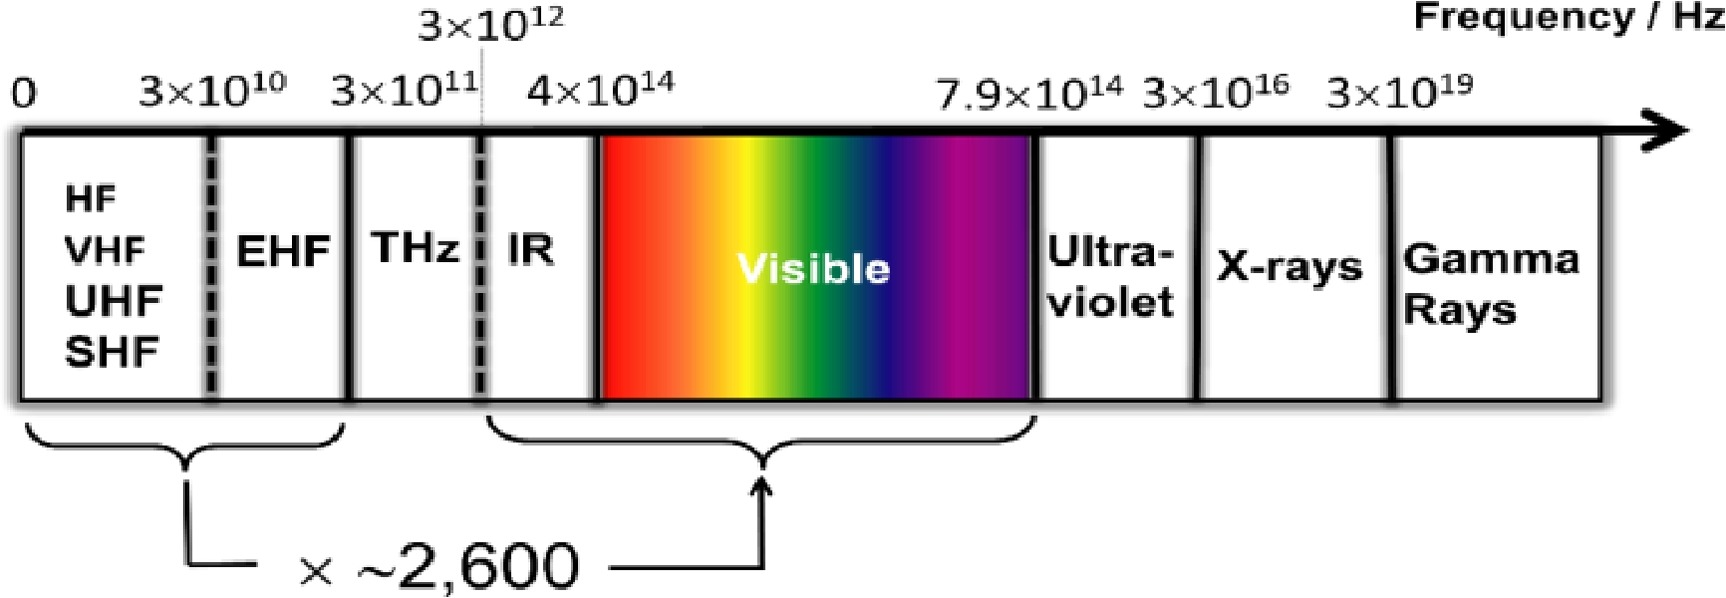
\includegraphics[width=\linewidth]{res/spectrum_li_fi.jpg}
    \caption{spectrum comparison. Source: \parencite{hass18}}
  \label{fig:spectrum_li_fi}
\end{figure}


%--------------------------------- Working --------------------------------


\subsection{Working of Li-Fi}


%------------------------ Modulation-Demodulation -------------------------
\subsubsection{Modulation-Demodulation}

According to \textcite{dimitrov12}, the system uses Orthogonal Frequency Division
Multiplexing(OFDM) for modulating the signals. As shown in the figure 4, first
the transmitting data is mapped to complex symbols X(l) by some modulation
scheme like M-QAM.  Then signals are summed using IFFT(Inverse Fast Fourier
Transformation).  Then signal is guarded after P/S conversion and transmitted
through light source.

At the receiver's end, the signals are converted from serial to parallel and
individual signals are extracted using FFT(Fast Fourier Transformation).
Signals are then demodulated and send to the receiver.

\begin{figure}[!h]
  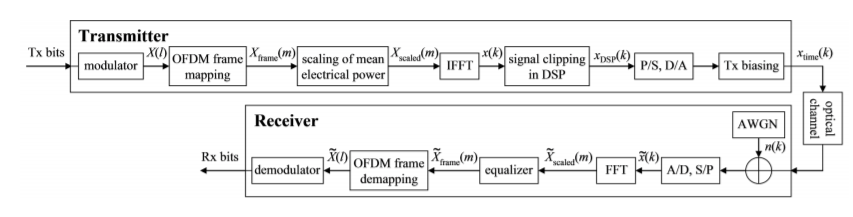
\includegraphics[width=\linewidth]{res/OFDM_li_fi.PNG}
    \caption{General OFDM. Source: \parencite{dimitrov12}}
  \label{fig:OFDM_li_fi}
\end{figure}


%---------------------------- Hardware -----------------------------
\subsubsection{Hardware Requirements}

\textcite{elgala09} states that LiFi requires two DSP(Digital Signal Processor)
boards, at transmitter and receiver ends respectively, one LED bulb and a
Photo-Diode reciever.\\ The Electric Signal from the transmitter are first
modulated using OFDM by the DSP board, installed between transmitter and the
LED.  The intensity of the LED to generate the signal is controlled by this
DSP.\\

At the other end, Photo-Diode receiver detects the high speed fluctuations of
the intensity of LED. DSP connected to Photo-Diode receiver decodes the OFDM
signals and transmits it to the receiver.  The fluctuations caused in LED are
so fast that it's impossible to detect them by naked eye, and hence serves the
purpose of normal LED.

\begin{figure}[!h]
  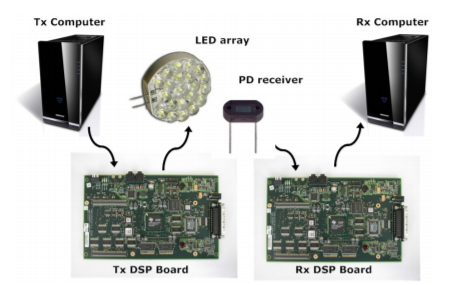
\includegraphics[width=\linewidth]{res/hardware_li_fi.PNG}
    \caption{simple OW system. Source: \parencite{elgala09}}
  \label{fig:hardware_li_fi}
\end{figure}



%----------------------------- Advantages -----------------------------

\subsection{Advantages}

\begin{description}
    
    \item [Speed] Data transmission speed can reach as high as 224 gigabits per
        second under light transmission.

    \item [Bandwidth] The unused bandwidth of 400THz in Visible Light Spectrum
        can be exploit for transmission. 

    \item [Cost and Availability]  There is no issue of initial setup and
        availability, the LEDs are much cheaper and can be used in place of
        fluorescent bulbs easily.
    
    \item [Security]  Light cannot penetrate through walls, and can be
        localized to the area of operation. Hence, provide secure environment
        for data transmission.
    
    \item [Efficiency] Energy consumption of LED is much less than other
        artificial light source and there is not much addition energy required
        for data transmission making it much efficient.
    
\end{description}


%------------------------ Misconceptions --------------------------------

\subsection{Misconceptions}

\begin{description}
    
    \item [It won't work in dark] As data is transmitted through light, one can
        think that we have to switch on the LED always, and we cannot keep the
        room dark. But these LEDs can be dimmed low enough that it will not be
        visible to human eye and still can be used for transmission.

    \item [It won't work in fog] The PD receiver can detect the mere
        fluctuations from the light source even if there is fog in-between.

    \item [It's not bidirectional] Li-Fi is a Fully duplex system and
        networked, hence handover as you move around in space.
    
    \item [Li-Fi doesn't work in sunlight] Li-Fi relies on fast change in light
        intensity, and not on slowly changing natural sources. Various filters
        can be used to decrease the interference from other sources.
    
\end{description}

%------------------------ Standardization -----------------------------
\subsection{Global light communication standards}

In 2019, IEEE announced formation of 802.11 bb task group which will develop
and ratify the Global standard for Li-Fi, opening the doors for the use of
technology at global level. 
The team aims to deliver the standards by mid 2021.


\printbibliography[heading=subbibliography]

\end{document}
